% Conversion y adaptacion de PMD_nextflow_17102022.pdf; ver README.md.
\ifdefined\PMDHandout
\documentclass[handout,aspectratio=169,10pt]{beamer}
\else
\documentclass[aspectratio=169,10pt]{beamer}
\fi
\usepackage[T1]{fontenc}
\usepackage[utf8]{inputenc}
\usepackage[spanish,es-nodecimaldot,es-noquoting]{babel}
\usepackage{lmodern,tgheros,booktabs,tabularx,listings,tikz}
\usetikzlibrary{arrows.meta,positioning}
\renewcommand{\familydefault}{\sfdefault}
\definecolor{uohblue}{HTML}{0075BA}
\definecolor{ink}{HTML}{162B3A}
\definecolor{muted}{HTML}{536978}
\definecolor{pale}{HTML}{EEF5F9}
\definecolor{codegreen}{HTML}{25784B}
\definecolor{codepurple}{HTML}{7B3979}
\definecolor{warm}{HTML}{B45C2C}
\setbeamercolor{normal text}{fg=ink,bg=white}
\setbeamercolor{structure}{fg=uohblue}
\setbeamercolor{frametitle}{fg=ink}
\setbeamercolor{framesubtitle}{fg=uohblue}
\setbeamercolor{block title}{fg=uohblue,bg=pale}
\setbeamercolor{block body}{fg=ink,bg=pale}
\setbeamerfont{frametitle}{size=\LARGE,series=\bfseries}
\setbeamerfont{framesubtitle}{size=\normalsize}
\setbeamertemplate{navigation symbols}{}
\setbeamertemplate{itemize items}[circle]
\setbeamercovered{invisible}
\setbeamersize{text margin left=8mm,text margin right=8mm}
\setbeamertemplate{frametitle}{\vspace{3mm}\insertframetitle\par{\usebeamerfont{framesubtitle}\usebeamercolor[fg]{framesubtitle}\insertframesubtitle\par}\vspace{1mm}}
\setbeamertemplate{footline}{\hbox to \paperwidth{\hspace{8mm}\color{muted}\scriptsize Alex Di Genova\enspace|\enspace Procesamiento Masivo de Datos\hfill Nextflow\quad\insertframenumber/\inserttotalframenumber\hspace{8mm}}\vspace{3mm}}
\lstdefinelanguage{Nextflow}{morekeywords={nextflow,enable,dsl,params,process,workflow,input,output,script,path,val,tuple,tag,stdout,include,from,as,true,false},sensitive=true,morecomment=[l]{//},morestring=[b]',morestring=[b]"}
\lstdefinestyle{nf}{language=Nextflow,basicstyle=\ttfamily\fontsize{8.2}{10}\selectfont,keywordstyle=\color{uohblue}\bfseries,commentstyle=\color{codegreen},stringstyle=\color{codepurple},backgroundcolor=\color{pale},columns=fullflexible,keepspaces=true,showstringspaces=false,breaklines=true,breakatwhitespace=true,tabsize=4,xleftmargin=5pt,xrightmargin=5pt}
\lstdefinestyle{shell}{style=nf,language=bash}
\lstset{style=nf}
\newcommand{\code}[1]{\texttt{\detokenize{#1}}}
\newcommand{\smallnote}[1]{\par\vspace{2pt}{\scriptsize\color{muted}#1\par}}
\tikzset{flow/.style={-{Latex[length=2mm]},thick,draw=uohblue},box/.style={draw=uohblue,fill=pale,rounded corners=2pt,minimum height=8mm,align=center,font=\small,inner sep=5pt}}
\hypersetup{pdftitle={Procesamiento Masivo de Datos: Nextflow},pdfauthor={Alex Di Genova},colorlinks=true,urlcolor=uohblue,linkcolor=uohblue}
\begin{document}
\begin{frame}[plain]
\begin{tikzpicture}[remember picture,overlay]
\node[anchor=north west,inner sep=0] at ([xshift=8mm,yshift=-5mm]current page.north west) {
\includegraphics[height=13mm]{assets/uoh.png}};
\node[anchor=north east,inner sep=0] at ([xshift=-8mm,yshift=-5mm]current page.north east) {
\includegraphics[width=49mm]{assets/ici.pdf}};
\fill[pale] (current page.south west) rectangle ([yshift=14mm]current page.south east);
\draw[uohblue,line width=1.3pt] ([xshift=8mm,yshift=14mm]current page.south west)--([xshift=45mm,yshift=14mm]current page.south west);
\node[anchor=north west,inner sep=0,text width=14cm] at ([xshift=8mm,yshift=-27mm]current page.north west) {{\fontsize{26}{30}\selectfont\bfseries Procesamiento Masivo de Datos\par}\vspace{3mm}{\fontsize{25}{29}\selectfont\color{uohblue}Nextflow\par}\vspace{2mm}{\large Flujos científicos escalables y reproducibles\par}\vspace{4mm}{\large Alex Di Genova\par}\vspace{2mm}{\color{muted}Universidad de O'Higgins\par}};
\node[anchor=south east,font=\small,text=muted] at ([xshift=-8mm,yshift=7mm]current page.south east) {Orquestación de pipelines};
\end{tikzpicture}
\end{frame}
\section{Introducción}
\begin{frame}{De datos genómicos a resultados}{Un flujo de procesos conectados}
\begin{center}
\begin{tikzpicture}[node distance=12mm]
\node[box] (a) {Datos}; \node[box,right=of a] (b) {Control de\\calidad}; \node[box,right=of b] (c) {Alineamiento}; \node[box,right=of c] (d) {Análisis}; \node[box,right=of d] (e) {Resultados};
\draw[flow] (a)--(b); \draw[flow] (b)--(c); \draw[flow] (c)--(d); \draw[flow] (d)--(e);
\end{tikzpicture}
\end{center}
\vspace{5mm}
\begin{itemize}[<+->]\setlength\itemsep{5pt}
\item \textbf{Reproducibilidad:} registrar datos, versiones y configuración.
\item \textbf{Escalabilidad:} procesar muchas muestras en un clúster o en la nube.
\item \textbf{Portabilidad:} adaptar la ejecución a distintas infraestructuras.
\item \textbf{Heterogeneidad:} aislar dependencias y asignar recursos por tarea.
\end{itemize}
\end{frame}
\begin{frame}{Un análisis genómico como flujo de datos}{De la muestra al análisis y almacenamiento}
\begin{columns}[T,onlytextwidth]
\column{.43\textwidth}\centering
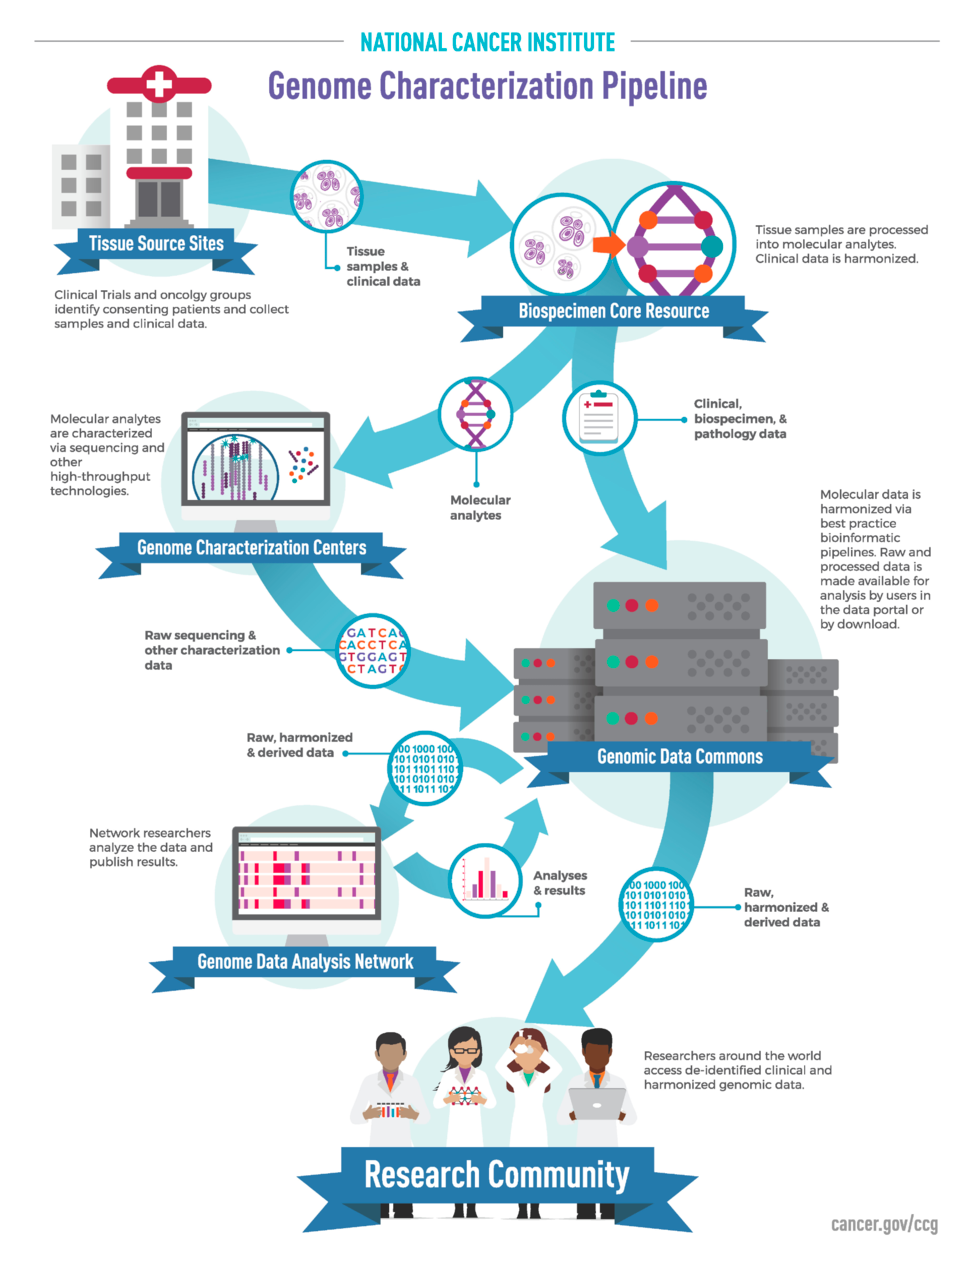
\includegraphics[height=59mm,keepaspectratio]{assets/genomica-original.png}
\column{.53\textwidth}
\begin{itemize}\setlength\itemsep{7pt}
\item Las muestras pasan por preparación, caracterización, análisis y almacenamiento.
\item Cada etapa produce datos que alimentan a otras tareas.
\item Un workflow expresa esas dependencias y coordina el procesamiento de múltiples muestras.
\end{itemize}
\end{columns}
\smallnote{Fuente: National Cancer Institute, Genome Characterization Pipeline.}
\end{frame}
\begin{frame}{Procesos conectados por canales}{Un flujo puede ramificarse y reunirse}
\begin{columns}[T,onlytextwidth]
\column{.56\textwidth}\centering
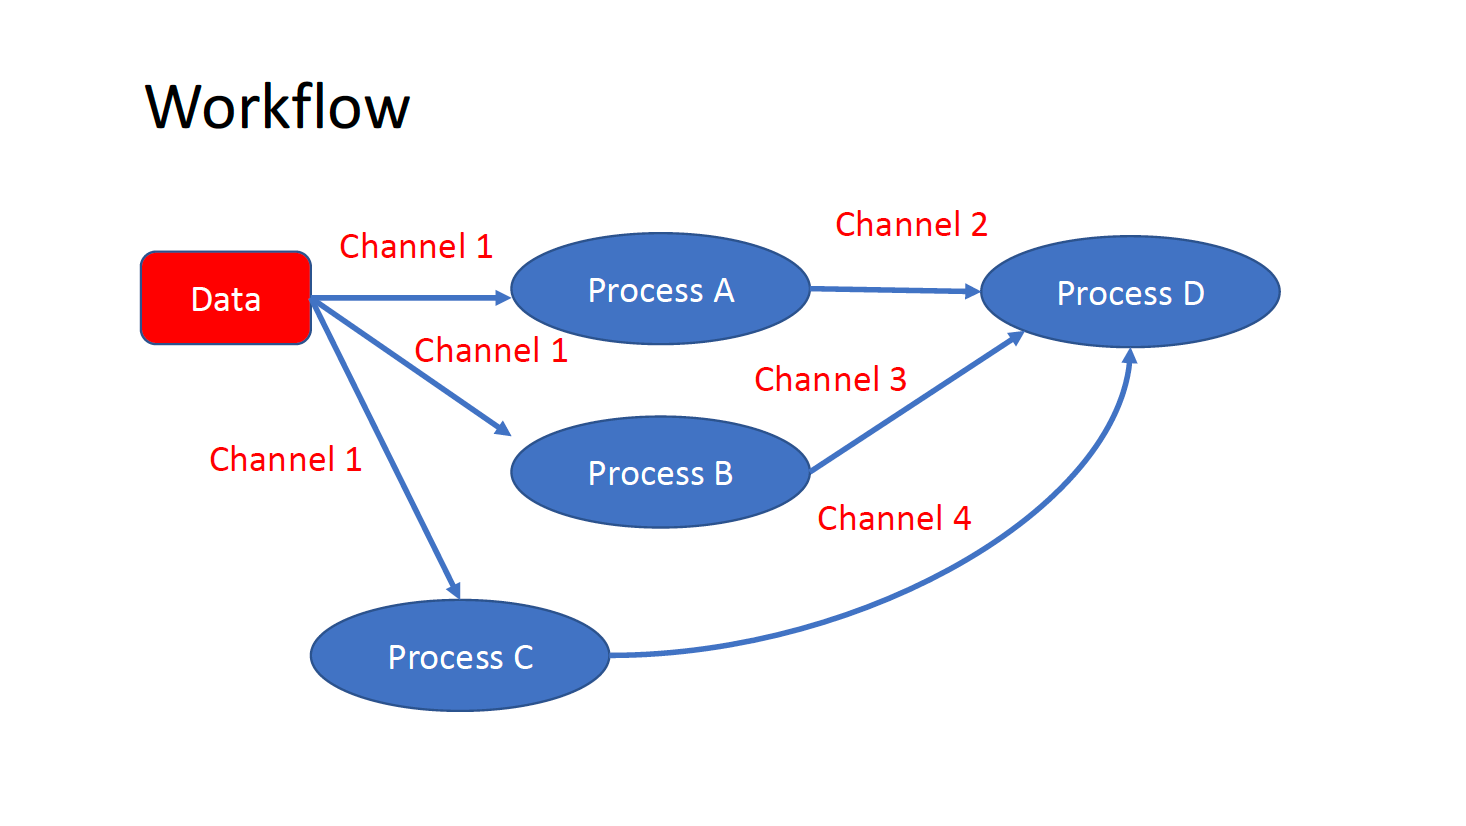
\includegraphics[width=\linewidth,height=53mm,keepaspectratio]{assets/flujo-canales-original.png}
\column{.40\textwidth}
\begin{itemize}\setlength\itemsep{6pt}
\item Los canales transportan valores entre etapas.
\item Un proceso puede recibir y producir tuplas con varios componentes.
\item Las ramas independientes pueden ejecutarse concurrentemente.
\end{itemize}
\end{columns}

\end{frame}

\begin{frame}{Un lenguaje para describir pipelines}{DSL: lenguaje específico de dominio}
\begin{itemize}[<+->]\setlength\itemsep{7pt}
\item Un DSL expresa tareas, entradas, salidas y dependencias del flujo.
\item \textbf{Nextflow} se basa en Groovy y usa programación orientada al flujo de datos.
\item Otras opciones incluyen \textbf{Snakemake} y \textbf{WDL}.
\item El motor programa las tareas cuando sus entradas están disponibles; las tareas independientes pueden ejecutarse en paralelo.
\end{itemize}
\end{frame}
\begin{frame}{Diseño de un pipeline}{Separar análisis, dependencias y ejecución}
\begin{enumerate}[<+->]\setlength\itemsep{8pt}
\item Escribir comandos en Bash, Python, R u otro lenguaje disponible.
\item Definir procesos y conectarlos mediante canales.
\item Especificar dependencias: contenedores o entornos Conda.
\item Configurar recursos y ejecutor: local, planificador HPC o nube.
\item Ejecutar y revisar resultados, registros y reportes.
\end{enumerate}
\end{frame}
\begin{frame}{Reproducibilidad entre plataformas}{Kallisto y Sleuth: ejecución nativa y con contenedor}
\begin{center}
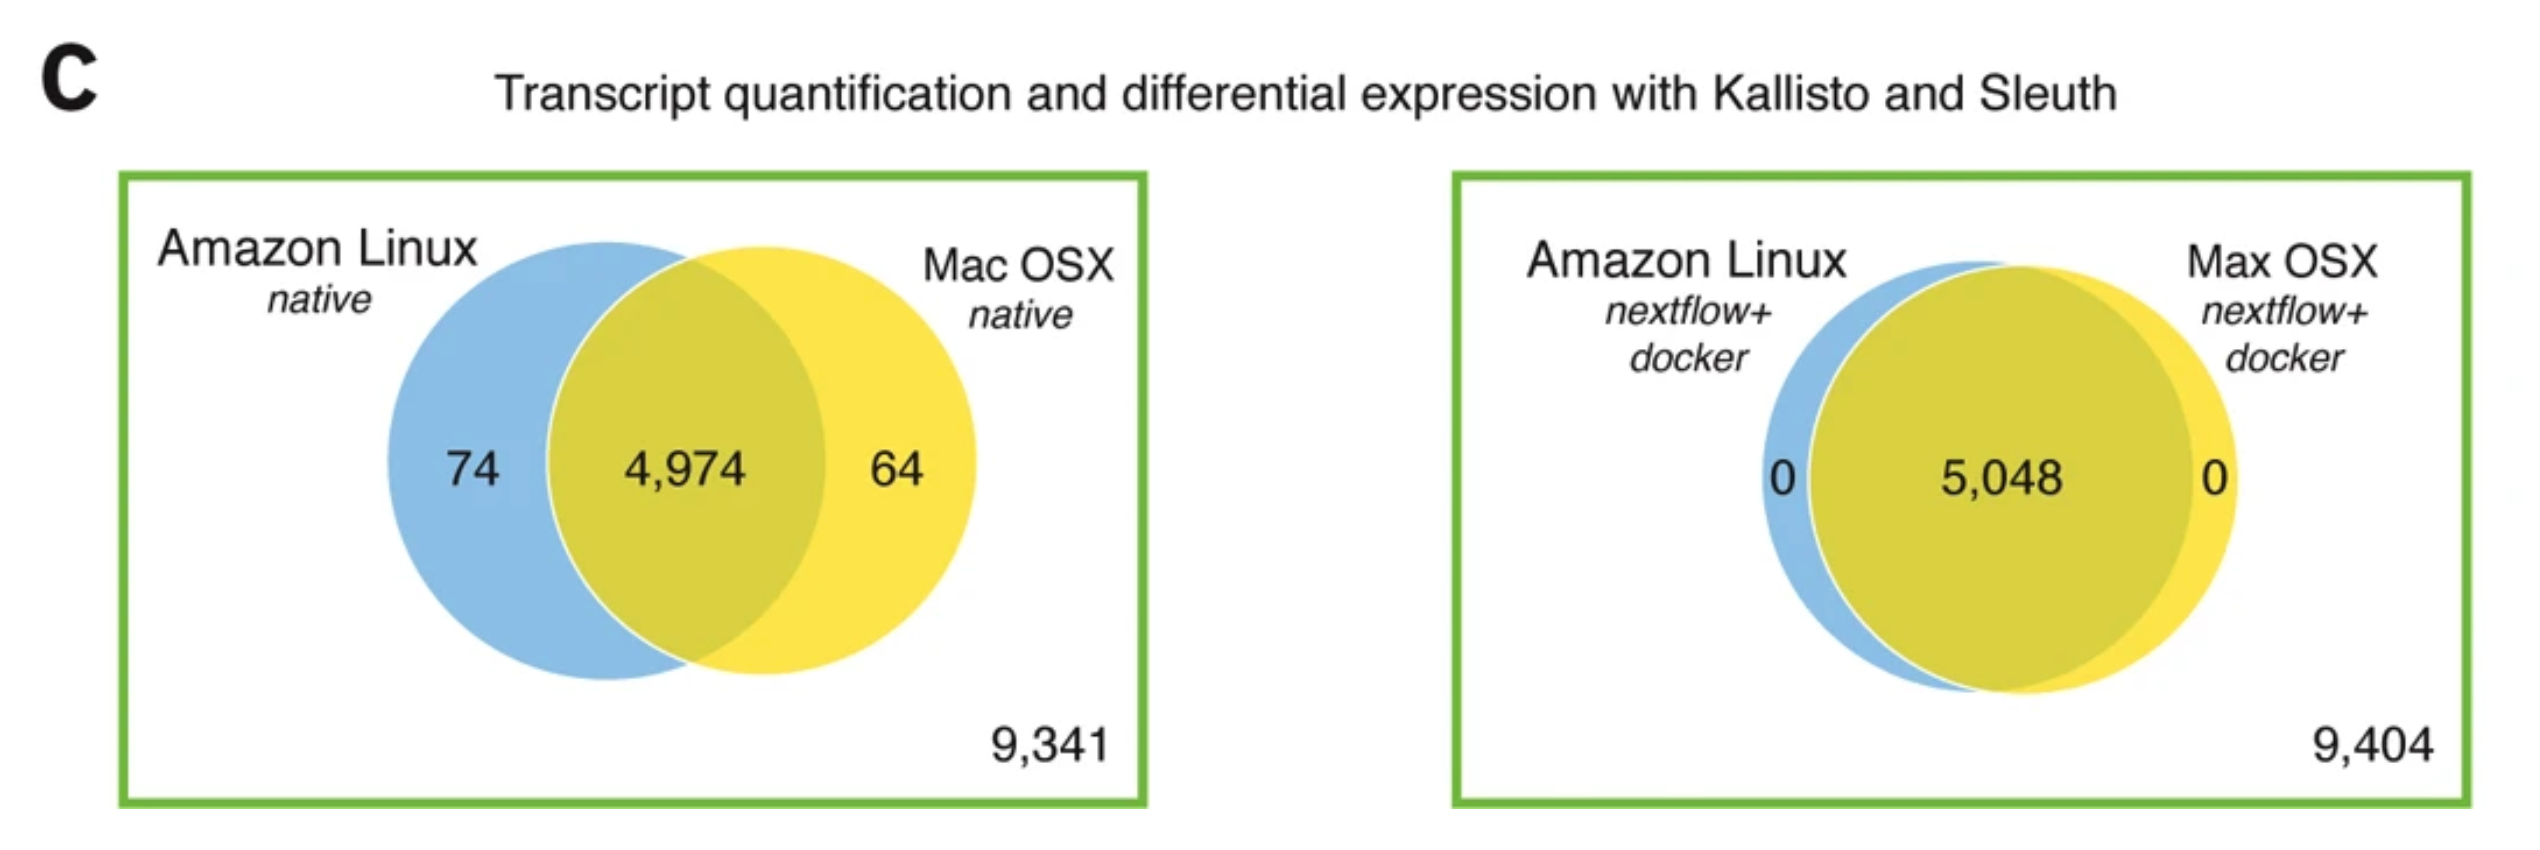
\includegraphics[width=.95\linewidth,height=40mm,keepaspectratio]{assets/paper-reproducibilidad.png}
\end{center}
\begin{itemize}\setlength\itemsep{3pt}
\item En ejecución nativa, 4.974 genes diferenciales coincidieron; 74 fueron exclusivos de Linux y 64 de macOS.
\item Con Nextflow y Docker, los 5.048 genes detectados coincidieron entre ambos entornos en este experimento.
\end{itemize}
\smallnote{Di Tommaso et al., \href{https://doi.org/10.1038/nbt.3820}{Nature Biotechnology, 2017, Fig. 1c}. La reproducibilidad también depende de los datos, parámetros y versiones.}
\end{frame}
\begin{frame}{Diseño de un programa Nextflow}{Del comando científico al flujo ejecutable}
\begin{center}
\begin{tikzpicture}[node distance=5mm and 9mm, every node/.style={align=center}]
\node[box,minimum width=38mm,minimum height=14mm] (code) {\textbf{1. Comandos}\\{\scriptsize Bash, Python, R, herramientas}};
\node[box,minimum width=42mm,minimum height=14mm,right=of code] (proc) {\textbf{2. Procesos y canales}\\{\scriptsize trimming $\to$ mapping $\to$ cuantificación}};
\node[box,minimum width=37mm,minimum height=14mm,right=of proc] (deps) {\textbf{3. Dependencias}\\{\scriptsize Conda, Docker, Apptainer}};
\node[box,minimum width=45mm,minimum height=14mm,below=12mm of code,xshift=28mm] (config) {\textbf{4. Configuración}\\{\scriptsize ejecutor, CPU, memoria, reintentos}};
\node[box,minimum width=38mm,minimum height=14mm,right=19mm of config] (run) {\textbf{5. Ejecución}\\{\scriptsize local, HPC o nube}};
\draw[flow] (code)--(proc); \draw[flow] (proc)--(deps);
\draw[flow] (deps.south) |- ([yshift=5mm]config.north) -- (config.north);
\draw[flow] (config)--(run);
\end{tikzpicture}
\end{center}
\smallnote{Las tareas se activan cuando sus entradas están disponibles y las tareas independientes pueden ejecutarse en paralelo.}
\end{frame}

\begin{frame}{Un flujo, distintas infraestructuras}{El ejecutor traduce tareas al entorno disponible}
\begin{center}
\begin{tikzpicture}[node distance=18mm]
\node[box] (nf) {Pipeline\\Nextflow}; \node[box,right=of nf] (ex) {Ejecutor};
\node[box,right=25mm of ex,yshift=15mm] (lo) {Local}; \node[box,right=25mm of ex] (sl) {HPC: SLURM, PBS, LSF}; \node[box,right=25mm of ex,yshift=-15mm] (cl) {Nube};
\draw[flow] (nf)--(ex); \draw[flow] (ex)--(lo); \draw[flow] (ex)--(sl); \draw[flow] (ex)--(cl);
\end{tikzpicture}
\end{center}
\vspace{5mm}
\begin{itemize}\item El acceso a datos, los recursos y las dependencias deben configurarse para cada entorno.\item Un clúster combina nodos de cómputo, red y un planificador de trabajos.\end{itemize}
\end{frame}
\begin{frame}{Dependencias y contenedores}{Empaquetar el entorno de cada herramienta}
\begin{columns}[T,onlytextwidth]
\column{.53\textwidth}
\begin{itemize}[<+->]\setlength\itemsep{7pt}
\item Una imagen reúne herramientas y bibliotecas con versiones definidas.
\item Docker y Apptainer/Singularity permiten usar imágenes en entornos compatibles.
\item Conda ofrece otra forma de gestionar dependencias.
\item El ejecutor y el sistema de contenedores se configuran por separado.
\end{itemize}
\column{.42\textwidth}
\begin{block}{Para reproducir un análisis}
Fijar versión del pipeline, imágenes y parámetros; conservar las versiones de los datos de entrada.
\end{block}
\end{columns}
\end{frame}
\begin{frame}{Arquitectura de ejecución}{Del DSL a las tareas}
\begin{columns}[T,onlytextwidth]
\column{.53\textwidth}\centering
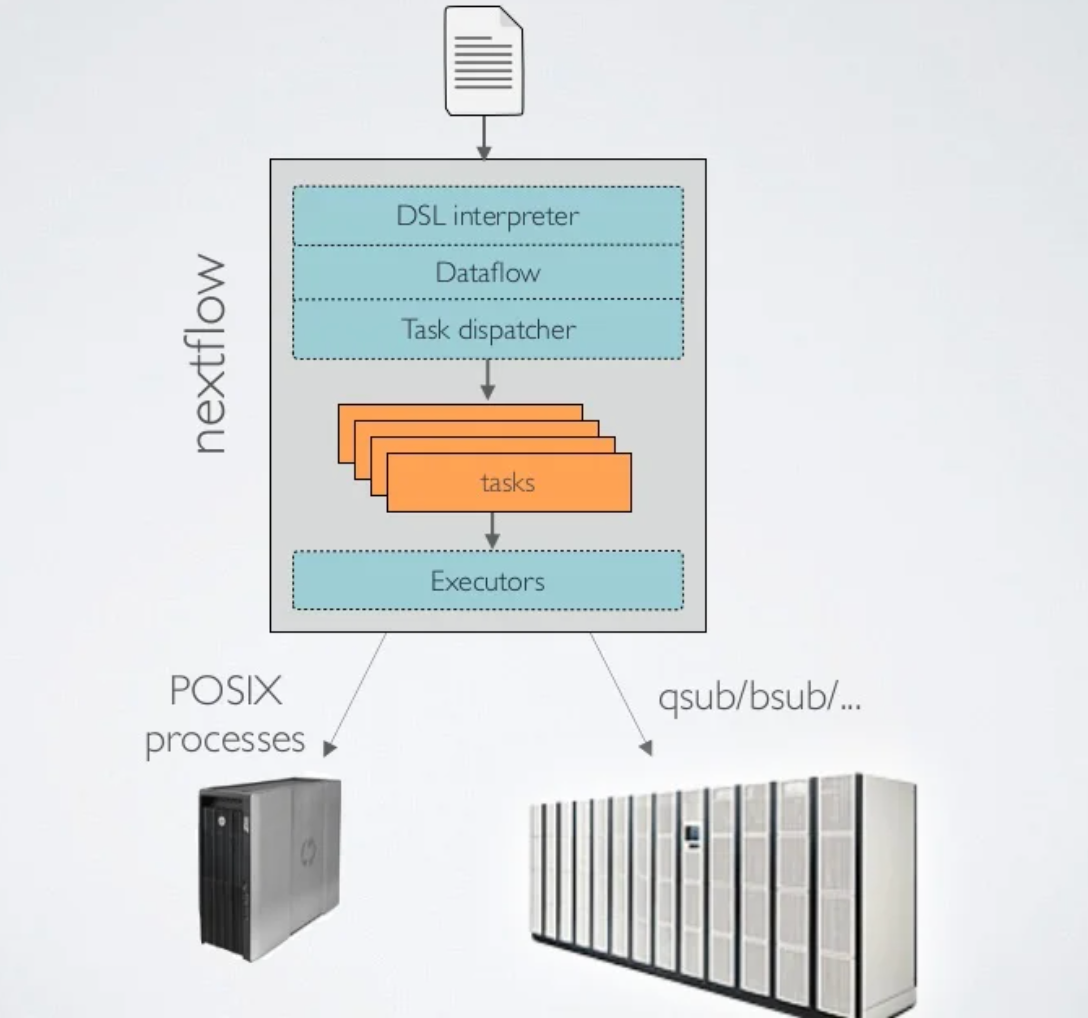
\includegraphics[height=60mm,keepaspectratio]{assets/arquitectura-original.png}
\column{.43\textwidth}
\begin{itemize}\setlength\itemsep{6pt}
\item Nextflow interpreta el flujo y determina las tareas listas.
\item El ejecutor las inicia localmente o las envía al planificador.
\item Los procesos y sus comandos se ejecutan en el entorno configurado.
\end{itemize}
\end{columns}

\end{frame}
\begin{frame}{Integración con infraestructura}{Ejemplo conceptual de despliegue}
\begin{columns}[T,onlytextwidth]
\column{.56\textwidth}\centering
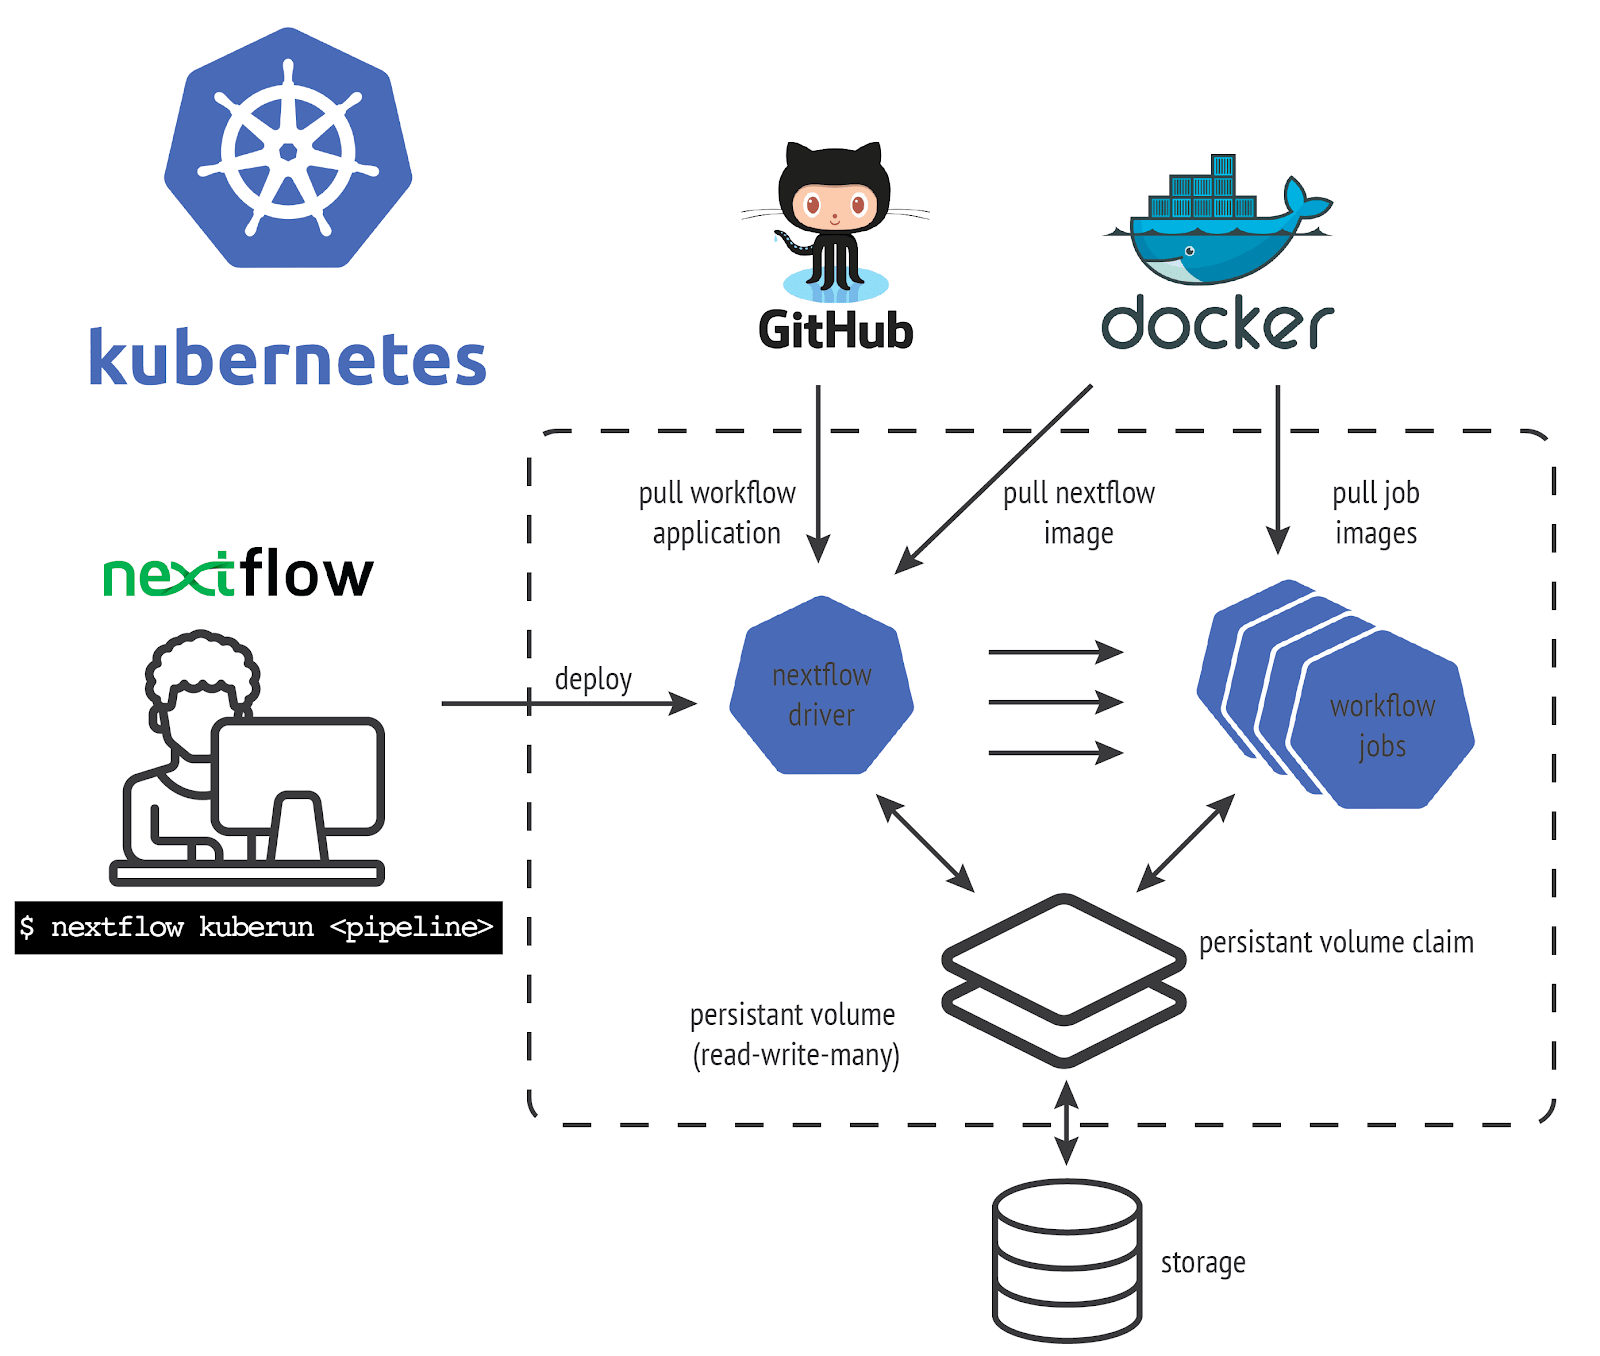
\includegraphics[width=\linewidth,height=56mm,keepaspectratio]{assets/nube-original.png}
\column{.40\textwidth}
\begin{itemize}\setlength\itemsep{6pt}
\item El flujo, las imágenes de software y los datos se gestionan como componentes distintos.
\item El entorno de cómputo recibe las tareas y accede al almacenamiento.
\item La configuración concreta depende de la plataforma y del almacenamiento disponible.
\end{itemize}
\end{columns}

\end{frame}

\begin{frame}{Un elemento de canal activa una tarea}{Paralelismo entre muestras}
\begin{columns}[T,onlytextwidth]
\column{.58\textwidth}\centering
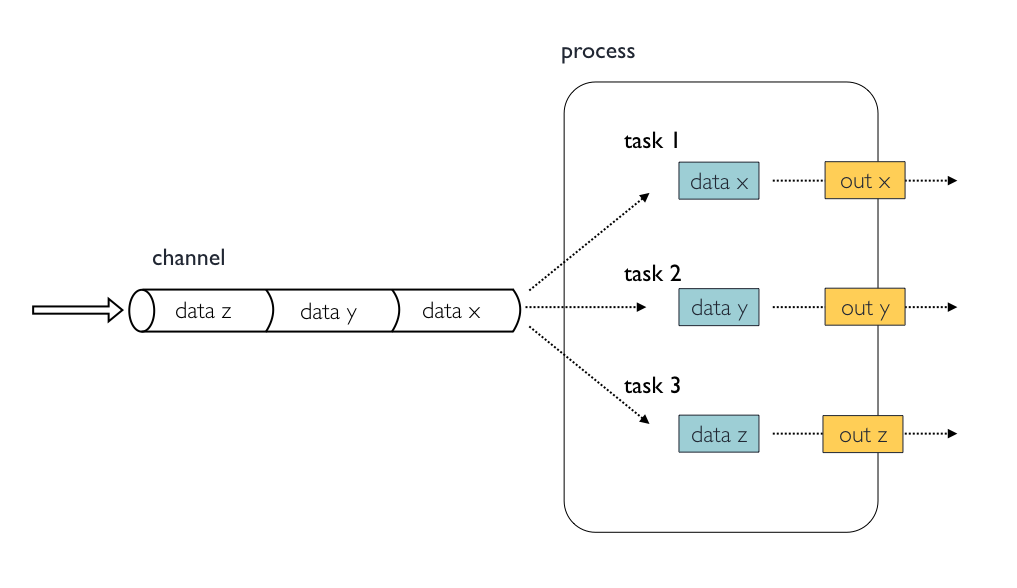
\includegraphics[width=\linewidth,height=56mm,keepaspectratio]{assets/canal-tareas.png}
\column{.38\textwidth}
\begin{itemize}\setlength\itemsep{6pt}
\item El proceso recibe elementos del canal y crea instancias de tarea.
\item Cada tarea tiene su directorio de trabajo y produce sus propias salidas.
\item El planificador puede ejecutar tareas listas simultáneamente según los recursos disponibles.
\end{itemize}
\end{columns}
\end{frame}
\begin{frame}{Imágenes y entornos de ejecución}{Dependencias reproducibles}
\begin{columns}[T,onlytextwidth]
\column{.48\textwidth}\centering
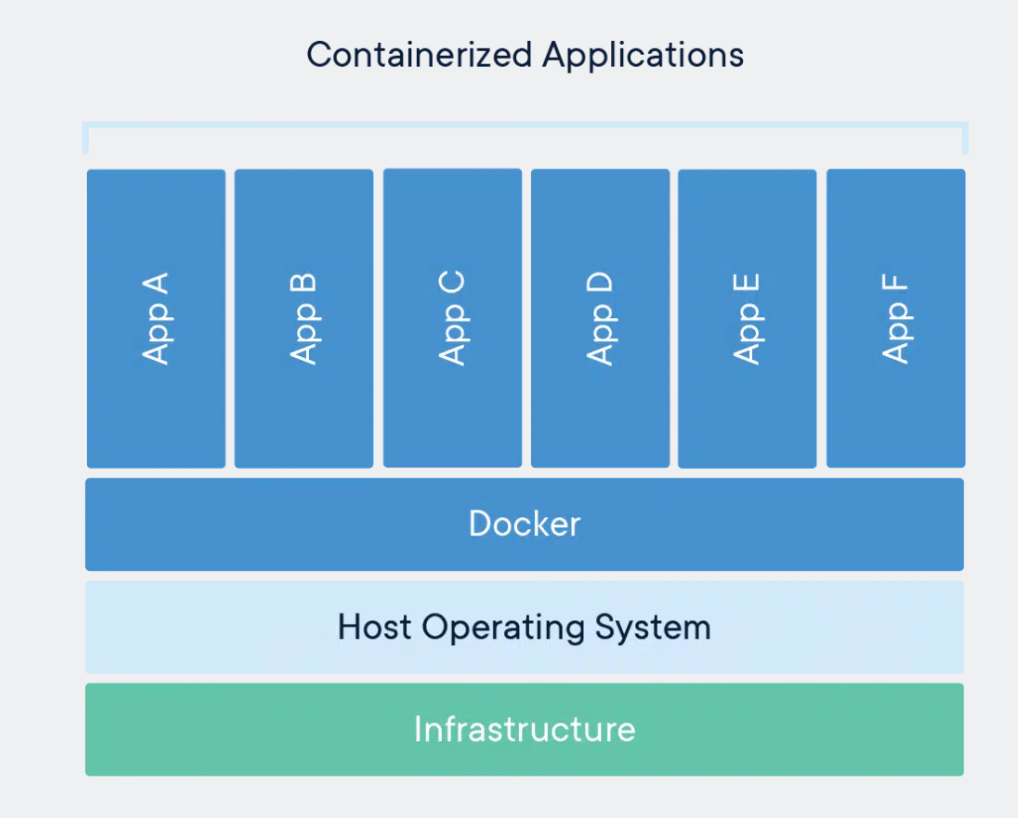
\includegraphics[height=47mm,keepaspectratio]{assets/contenedores-capas.png}
\column{.48\textwidth}\centering

\includegraphics[width=\linewidth,height=47mm,keepaspectratio]{assets/contenedores-flujo.png}
\end{columns}
\vspace{2mm}
\begin{itemize}\item Cada proceso puede usar una imagen con las versiones de herramientas y bibliotecas que necesita.\item Fijar una etiqueta inmutable o un digest ayuda a reconstruir el entorno.\end{itemize}
\end{frame}
\begin{frame}{Interpretar métricas por proceso}{Detectar cuellos de botella}
\begin{columns}[T,onlytextwidth]
\column{.33\textwidth}\centering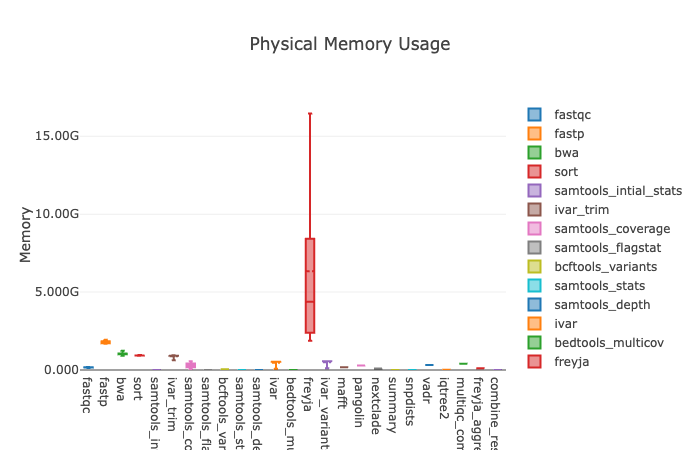
\includegraphics[width=\linewidth]{assets/uso-memoria.png}\\{\scriptsize Memoria física}
\column{.33\textwidth}\centering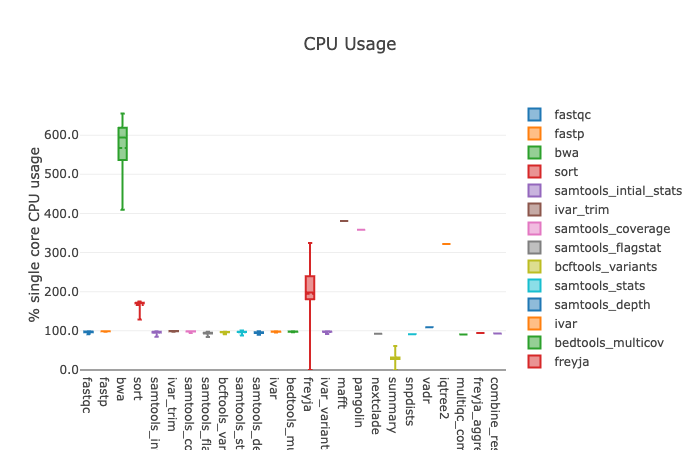
\includegraphics[width=\linewidth]{assets/uso-cpu.png}\\{\scriptsize Uso de CPU}
\column{.33\textwidth}\centering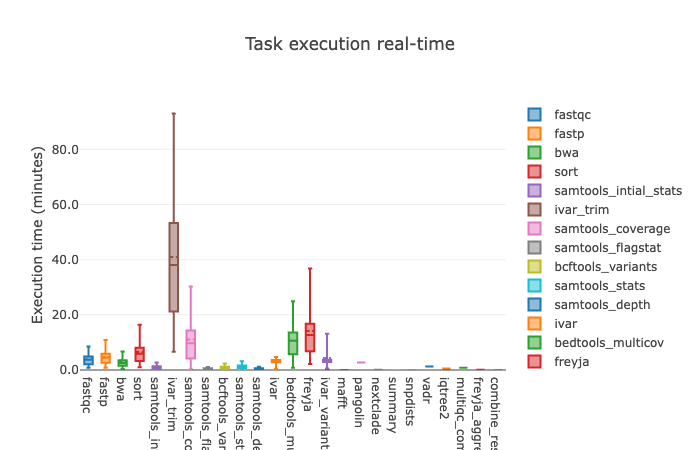
\includegraphics[width=\linewidth]{assets/tiempo-tareas.png}\\{\scriptsize Tiempo por tarea}
\end{columns}
\vspace{3mm}
\begin{itemize}\item Comparar tareas y procesos permite ajustar memoria, CPU y tiempo solicitados.\item Las métricas disponibles dependen del ejecutor y del entorno de ejecución.\end{itemize}
\end{frame}

\begin{frame}[fragile]{De la pesadilla de dependencias a un flujo reproducible}{Cada herramienta necesita su propio entorno}
\begin{columns}[T,onlytextwidth]
\column{.47\textwidth}
\begin{block}{Un análisis puede necesitar}
FastQC, Trim Galore, STAR, SAMtools, GATK, MultiQC, R y bibliotecas específicas.
\end{block}
\begin{itemize}\item Versiones incompatibles y múltiples instalaciones complican la ejecución.\end{itemize}
\column{.49\textwidth}
\begin{block}{Con Nextflow y contenedores}
El workflow declara las tareas; las imágenes aportan las herramientas y dependencias que cada una necesita.
\end{block}
\begin{lstlisting}[style=shell]
nextflow run org/pipeline \
  -r v1.0 -profile singularity \
  --input samplesheet.csv
\end{lstlisting}
\end{columns}
\smallnote{Ejemplo esquemático: el perfil y los parámetros dependen del pipeline; el motor de contenedores debe estar disponible.}
\end{frame}

\section{Uso de pipelines}
\begin{frame}[fragile]{Ejecutar un pipeline}{Repositorio, revisión y perfil}
\begin{lstlisting}[style=shell]
nextflow run digenoma-lab/longreadstats \
    -r v1.0dev -profile singularity \
    --input samplesheet.csv
\end{lstlisting}
\begin{itemize}[<+->]\setlength\itemsep{6pt}
\item \code{digenoma-lab/longreadstats}: repositorio del pipeline.
\item \code{-r}: revisión, etiqueta o rama; fijar una versión favorece la reproducibilidad.
\item \code{-profile}: configuración proporcionada por el pipeline.
\item \code{--input}: parámetro del pipeline; su formato depende del proyecto.
\end{itemize}
\smallnote{Consultar el repositorio para verificar revisiones, perfiles y parámetros disponibles.}
\end{frame}
\begin{frame}[fragile]{Configuración y reanudación}{Adaptar recursos sin modificar el análisis}
\begin{columns}[T,onlytextwidth]
\column{.49\textwidth}
\lstinputlisting[style=nf,basicstyle=\ttfamily\fontsize{8}{9.5}\selectfont]{examples/nextflow.config}
\column{.47\textwidth}
\begin{itemize}\setlength\itemsep{6pt}
\item Seleccionar un perfil con \code{-profile slurm}.
\item Cada proceso puede definir sus propios recursos.
\item \code{-resume} reutiliza tareas en caché cuando es posible; conservar el directorio \code{work} y la caché.
\end{itemize}
\end{columns}
\end{frame}
\begin{frame}[fragile]{Reportes de ejecución}{Resumen y trazabilidad del workflow}
\begin{center}
\begin{tikzpicture}[x=1cm,y=1cm,scale=.83,transform shape]
  \fill[pale,rounded corners=2pt] (0,0) rectangle (12.4,3.75);
  \fill[ink,rounded corners=2pt] (0,3.18) rectangle (12.4,3.75);
  \fill[ink] (0,3.18) rectangle (12.4,3.35);
  \node[anchor=west,text=white,font=\bfseries\small] at (.25,3.47) {Nextflow Report};
  \node[anchor=east,text=white,font=\scriptsize] at (12.15,3.47) {Summary \quad Resources \quad Tasks};
  \node[anchor=west,font=\bfseries\small,text=ink] at (.28,2.77) {Comando};
  \node[anchor=west,font=\ttfamily\small,text=ink] at (3.65,2.77) {nextflow run main.nf -profile singularity};
  \draw[muted!25] (.28,2.52)--(12.1,2.52);
  \node[anchor=west,font=\bfseries\small,text=ink] at (.28,2.15) {Versión del pipeline};
  \node[anchor=west,font=\ttfamily\small,text=ink] at (3.65,2.15) {v1.0};
  \node[anchor=west,font=\bfseries\small,text=ink] at (6.3,2.15) {Perfil};
  \node[anchor=west,font=\ttfamily\small,text=ink] at (8.15,2.15) {singularity};
  \draw[muted!25] (.28,1.88)--(12.1,1.88);
  \node[anchor=west,font=\bfseries\small,text=ink] at (.28,1.50) {Directorio de trabajo};
  \node[anchor=west,font=\ttfamily\small,text=ink] at (3.65,1.50) {proyecto/work};
  \draw[muted!25] (.28,1.23)--(12.1,1.23);
  \node[anchor=west,font=\bfseries\small,text=ink] at (.28,.84) {Recursos};
  \node[anchor=west,font=\small,text=ink] at (3.65,.84) {tiempo, CPU y memoria por proceso};
  \node[anchor=west,font=\scriptsize,text=muted] at (.28,.28) {Ejemplo esquemático de un reporte de ejecución};
\end{tikzpicture}
\end{center}
\vspace{-3mm}
\begin{lstlisting}[style=shell,basicstyle=\ttfamily\fontsize{9}{11}\selectfont]
nextflow run main.nf -with-report reporte.html
\end{lstlisting}
\end{frame}
\section{Procesos y canales}
\begin{frame}{Procesos y canales}{La unidad de ejecución es una tarea}
\begin{itemize}[<+->]\setlength\itemsep{6pt}
\item Un \textbf{proceso} declara entradas, salidas y el comando que se ejecuta.
\item Un \textbf{canal} transporta valores o rutas entre procesos.
\item Cada elemento de entrada puede generar una tarea; las tareas trabajan en directorios aislados.
\item El flujo conecta procesos explícitamente; el motor resuelve dependencias y planifica tareas.
\end{itemize}
\end{frame}
\begin{frame}[fragile]{Primer proceso}{Contar líneas de archivos FASTQ comprimidos}
\begin{lstlisting}
process CONTAR_LINEAS {
    tag "${read.name}"
    input:
    path read
    output:
    tuple val(read.name), path('lineas.txt')
    script:
    """
    gzip -cd '${read}' | wc -l > lineas.txt
    """
}
\end{lstlisting}
\smallnote{Cada tarea escribe su propio \code{lineas.txt}. El resultado es una tupla con nombre y archivo.}
\end{frame}
\begin{frame}[fragile]{Conectar el proceso}{Crear un canal y observar la salida}
\begin{lstlisting}
params.reads = 'data/*.fq.gz'
workflow {
    reads = Channel.fromPath(params.reads, checkIfExists: true)
    CONTAR_LINEAS(reads).view { nombre, archivo ->
        "${nombre}: ${archivo.text.trim()} lineas"
    }
}
\end{lstlisting}
\begin{lstlisting}[style=shell]
nextflow run examples/conteo.nf --reads 'data/*.fq.gz'
\end{lstlisting}
\smallnote{Archivo completo: \code{examples/conteo.nf}. En FASTQ válido, cuatro líneas representan una lectura; el conteo es de líneas.}
\end{frame}
\begin{frame}[fragile]{Un flujo con dos etapas}{Índice compartido y cuantificación por muestra}
\begin{lstlisting}
workflow {
    referencia = Channel.fromPath(params.ref, checkIfExists: true)
    pares = Channel.fromFilePairs(params.reads, checkIfExists: true)
    indice = INDEX(referencia.first())
    QUANT(indice, pares)
}
\end{lstlisting}
\begin{itemize}\setlength\itemsep{6pt}
\item \code{INDEX} produce un índice; \code{QUANT} usa ese índice con cada par de lecturas.
\item \code{first()} produce un valor reutilizable: el ejemplo supone exactamente una referencia.
\item Los procesos declaran sus entradas y salidas; a continuación se presenta el ejemplo con Salmon.
\end{itemize}
\end{frame}
\begin{frame}[fragile]{Ejemplo Salmon: construir el índice}{Una referencia de transcriptoma}
\begin{lstlisting}
process INDEX {
    cpus 2
    input:
    path transcriptome
    output:
    path 'indice'
    script:
    """
    salmon index -t '${transcriptome}' -i indice -p ${task.cpus}
    """
}
\end{lstlisting}
\smallnote{El proceso recibe un archivo de referencia y produce un directorio con el índice. Código completo: \code{examples/salmon.nf}.}
\end{frame}
\begin{frame}[fragile]{Ejemplo Salmon: cuantificar cada muestra}{Una tarea por par de lecturas}
\begin{lstlisting}
process QUANT {
    cpus 2
    input:
    path indice
    tuple val(sample), path(reads)
    output:
    tuple val(sample), path('quant')
    script:
    """
    salmon quant -i '${indice}' -l A -1 '${reads[0]}' \\
        -2 '${reads[1]}' -p ${task.cpus} -o quant
    """
}
\end{lstlisting}
\smallnote{La salida conserva el ID junto al directorio de resultados. El ejemplo requiere Salmon y datos compatibles.}
\end{frame}

\begin{frame}[fragile]{Crear canales}{Valores y archivos}
\begin{lstlisting}
Channel.of('A', 'B', 'C')       // tres elementos
Channel.of(['A', 'B', 'C'])     // un elemento: una lista
Channel.fromPath('data/*.fq.gz', checkIfExists: true)
Channel.fromFilePairs('data/*_{1,2}.fq.gz', checkIfExists: true)
\end{lstlisting}
\vspace{2mm}
\begin{itemize}\setlength\itemsep{6pt}
\item \code{val} entrega un valor; \code{path} prepara archivos para la tarea.
\item \code{fromFilePairs} emite \code{[id, [read1, read2]]} por muestra.
\item Las comillas en Bash evitan que el shell expanda el patrón antes de Nextflow.
\end{itemize}
\end{frame}
\begin{frame}[fragile]{Un proceso por par de lecturas}{Mantener el identificador junto a sus archivos}
\begin{lstlisting}
process MOSTRAR_PARES {
    input:
    tuple val(sample), path(reads)
    output:
    stdout
    script:
    """
    printf '%s: %s %s\n' '${sample}' '${reads[0]}' '${reads[1]}'
    """
}
workflow {
    pares = Channel.fromFilePairs(params.reads, checkIfExists: true)
    MOSTRAR_PARES(pares).view()
}
\end{lstlisting}
\smallnote{Código completo: \code{examples/pares.nf}. La tarea solo muestra nombres; sustituir el comando por la herramienta de interés.}
\end{frame}
\begin{frame}[fragile]{Una tabla de muestras}{Construir tuplas a partir de CSV}
\begin{lstlisting}[basicstyle=\ttfamily\fontsize{8.4}{10}\selectfont]
sampleId,read1,read2
muestraA,data/muestraA_1.fq.gz,data/muestraA_2.fq.gz
muestraB,data/muestraB_1.fq.gz,data/muestraB_2.fq.gz
\end{lstlisting}
\begin{lstlisting}
muestras = Channel.fromPath(params.sheet, checkIfExists: true)
    .splitCsv(header: true)
    .map { row -> tuple(row.sampleId, file(row.read1), file(row.read2)) }
MOSTRAR_MUESTRA(muestras)
\end{lstlisting}
\smallnote{Código completo: \code{examples/muestras.nf}. Las rutas relativas se interpretan desde el directorio de ejecución.}
\end{frame}
\begin{frame}{Anatomía de un canal}{Elementos, tuplas y cardinalidad}
\begin{center}
\begin{tikzpicture}[node distance=8mm]
\node[box] (a) {\texttt{[A, R1, R2]}}; \node[box,right=of a] (b) {\texttt{[B, R1, R2]}}; \node[box,right=of b] (c) {\texttt{[C, R1, R2]}};
\node[below=8mm of b,align=center] {Un canal con tres elementos\\cada elemento es una tupla de tres campos};
\end{tikzpicture}
\end{center}
\vspace{3mm}
\begin{itemize}\item Mantener ID y archivos en una sola tupla conserva la asociación entre ellos.\item Una lista dentro de un elemento es distinta de varios elementos independientes.\end{itemize}
\end{frame}
\begin{frame}[fragile]{Crear canales: \texttt{of}, \texttt{value} y \texttt{fromPath}}{Cuántos elementos se emiten}
\begin{lstlisting}
channel.of('A', 'B', 'C').view()       // A  B  C: tres elementos
channel.of(['A', 'B', 'C']).view()     // [A, B, C]: un elemento
channel.value('ref.fa')                // un valor reutilizable
channel.fromPath('data/*.fq.gz', checkIfExists: true).view()
\end{lstlisting}
\begin{itemize}\setlength\itemsep{6pt}
\item \code{of} emite cada argumento; \code{value} crea un canal de valor.
\item \code{fromPath} busca archivos que correspondan al patrón y emite rutas.
\item Un canal de valor puede reutilizarse para cada elemento de un canal de cola.
\end{itemize}
\end{frame}
\begin{frame}[fragile]{Leer pares y tablas}{\texttt{fromFilePairs} y \texttt{splitCsv}}
\begin{lstlisting}
channel.fromFilePairs('data/*_{1,2}.fq.gz').view()
// [muestraA, [muestraA_1.fq.gz, muestraA_2.fq.gz]]

channel.fromPath('examples/muestras.csv')
    .splitCsv(header: true)
    .map { row -> tuple(row.sampleId, file(row.read1), file(row.read2)) }
    .view()
// [muestraA, ruta/a/muestraA_1.fq.gz, ruta/a/muestraA_2.fq.gz]
\end{lstlisting}
\smallnote{\code{flat: true} en \code{fromFilePairs} emite ID y archivos en una tupla plana. Las rutas mostradas son esquemáticas.}
\end{frame}
\begin{frame}[fragile]{Transformar y filtrar}{\texttt{map}, \texttt{filter} y closures}
\begin{lstlisting}
channel.of(['A', 12], ['B', 5], ['C', 20])
    .filter { id, n -> n >= 10 }
    .map { id, n -> tuple(id, n * 2) }
    .view()
// [A, 24]
// [C, 40]
\end{lstlisting}
\begin{itemize}\item \code{filter} conserva elementos que cumplen el predicado.\item \code{map} transforma cada elemento; \code{it} representa el argumento cuando se omite su nombre.\item \code{view} permite inspeccionar el contenido del canal.\end{itemize}
\end{frame}
\begin{frame}[fragile]{Reordenar tuplas con \texttt{map}}{Cambiar forma sin perder asociación}
\begin{lstlisting}
channel.of(['A', 'A_1.fq', 'A_2.fq'],
           ['B', 'B_1.fq', 'B_2.fq'])
    .map { id, r1, r2 -> tuple(id, [r1, r2]) }
    .view()
// [A, [A_1.fq, A_2.fq]]
// [B, [B_1.fq, B_2.fq]]
\end{lstlisting}
\smallnote{El resultado tiene dos campos: un ID y una lista con dos nombres. Para entradas \code{path}, usar objetos archivo en lugar de cadenas.}
\end{frame}
\begin{frame}[fragile]{\texttt{flatten}: separar listas anidadas}{Más elementos, menos estructura}
\begin{lstlisting}
channel.of(['A', ['A_1.fq', 'A_2.fq']])
    .flatten()
    .view()
// A
// A_1.fq
// A_2.fq
\end{lstlisting}
\begin{itemize}\item \code{flatten} desanida recursivamente las listas y emite sus valores.\item Puede destruir la asociación entre muestra y archivos: usarlo solo si esa estructura ya no es necesaria.\end{itemize}
\end{frame}
\begin{frame}[fragile]{\texttt{collect} frente a \texttt{toList}}{Un solo elemento de salida, distinta estructura}
\begin{lstlisting}
channel.of(['A', 1], ['B', 2]).collect().view()
// [A, 1, B, 2]
channel.of(['A', 1], ['B', 2]).toList().view()
// [[A, 1], [B, 2]]
channel.of(['A', 1], ['B', 2]).collect(flat: false).view()
// [[A, 1], [B, 2]]
\end{lstlisting}
\smallnote{Ambos esperan el cierre. En entrada vacía, \code{collect()} no emite y \code{toList()} emite \code{[]}. El orden depende del canal de entrada.}
\end{frame}
\begin{frame}[fragile]{Ordenar o concatenar}{\texttt{toSortedList} y \texttt{concat}}
\begin{lstlisting}
channel.of('C', 'A', 'B').toSortedList().view()
// [A, B, C]

channel.of('A', 'B').concat(channel.of('C', 'D')).view()
// A, B, C, D
\end{lstlisting}
\begin{itemize}\item \code{toSortedList} reúne todos los elementos y entrega una lista ordenada.\item \code{concat} consume un canal después del otro; no forma pares ni producto cartesiano.\item Ordenar puede ser necesario antes de comparar resultados de tareas concurrentes.\end{itemize}
\end{frame}
\begin{frame}[fragile]{\texttt{combine}: todas las combinaciones}{Muestras por regiones genómicas}
\begin{lstlisting}
muestras = channel.of('A', 'B')
regiones = channel.of('chr1', 'chr2')
muestras.combine(regiones).view()
// [A, chr1]  [A, chr2]  [B, chr1]  [B, chr2]
\end{lstlisting}
\begin{itemize}\item Sin clave, produce el producto cartesiano: dos muestras por dos regiones generan cuatro elementos.\item Con \code{by: 0}, combina tuplas que comparten la clave de la posición 0; admite múltiples coincidencias por clave.\end{itemize}
\end{frame}
\begin{frame}[fragile]{\texttt{join}: asociar por identificador}{Un archivo BAM con su índice}
\begin{lstlisting}
bam = channel.of(['A', 'A.bam'], ['B', 'B.bam'])
bai = channel.of(['A', 'A.bai'], ['B', 'B.bai'])
bam.join(bai, failOnDuplicate: true).view()
// [A, A.bam, A.bai]
// [B, B.bam, B.bai]
\end{lstlisting}
\smallnote{Por defecto usa la primera posición y descarta claves sin pareja. \code{join} no implementa el producto cartesiano de claves duplicadas; para ello usar \code{combine(by: 0)}.}
\end{frame}
\begin{frame}[fragile]{\texttt{groupTuple}: reunir por clave}{Combinar lanes de una muestra}
\begin{lstlisting}
channel.of(['A', 'A_L1.fq'], ['B', 'B_L1.fq'],
           ['A', 'A_L2.fq'])
    .groupTuple()
    .view()
// [A, [A_L1.fq, A_L2.fq]]
// [B, [B_L1.fq]]
\end{lstlisting}
\begin{itemize}\item Agrupa los valores de las tuplas según su clave, por defecto el primer campo.\item Sin tamaño conocido, espera el cierre del canal; \code{size: n} permite emitir grupos completos antes.\end{itemize}
\end{frame}
\begin{frame}[fragile]{Funciones y closures de Groovy}{Transformaciones reutilizables}
\begin{lstlisting}
def etiqueta(id, n) {
    return "${id}: ${n} lecturas"
}
workflow {
    channel.of(['A', 100], ['B', 75])
        .map { id, n -> etiqueta(id, n) }
        .view()
}
// A: 100 lecturas
// B: 75 lecturas
\end{lstlisting}
\smallnote{Una función retorna un valor; un proceso declara una tarea ejecutable. La closure de \code{map} se aplica a cada elemento.}
\end{frame}
\begin{frame}[fragile]{Leer una lista de archivos}{\texttt{splitText} y conversión a rutas}
\begin{lstlisting}
// archivos.txt contiene una ruta por linea
channel.fromPath('examples/archivos.txt', checkIfExists: true)
    .splitText()
    .map { linea -> linea.trim() }
    .filter { linea -> linea && !linea.startsWith('#') }
    .map { ruta -> file(ruta, checkIfExists: true) }
    .view()
// /.../data/muestraA_1.fq.gz
// /.../data/muestraB_1.fq.gz
\end{lstlisting}
\smallnote{\code{splitText()} entrega una línea por elemento; \code{trim()} quita espacios y salto de línea. Las rutas relativas se resuelven desde el directorio de ejecución.}
\end{frame}
\begin{frame}[fragile]{Leer una tabla TSV}{Seleccionar columnas y añadir una ruta base}
\begin{lstlisting}
params.bam_dir = 'data/bam'
channel.fromPath('muestras.tsv', checkIfExists: true)
    .splitCsv(header: true, sep: '\t')
    .map { row ->
        def bam = file("${params.bam_dir}/${row.bam}")
        tuple(row.sample, bam, file("${bam}.bai"))
    }
    .view()
// [A, /.../data/bam/A.bam, /.../data/bam/A.bam.bai]
\end{lstlisting}
\smallnote{Ejemplo con columnas \code{sample} y \code{bam}, separadas por tabulación: se conserva el identificador junto al BAM y su índice. No comprueba aquí la existencia de ambos archivos.}
\end{frame}
\begin{frame}[fragile]{\texttt{flatMap}: expandir sin perder la clave}{Una tarea por región de cada muestra}
\begin{lstlisting}
channel.of(['A', ['chr1', 'chr2']], ['B', ['chr1']])
    .flatMap { id, regiones ->
        regiones.collect { chr -> tuple(id, chr) }
    }
    .view()
// [A, chr1]  [A, chr2]  [B, chr1]
\end{lstlisting}
\begin{itemize}\item La closure retorna una lista de tuplas; \code{flatMap} emite cada tupla.\item Se conserva el ID para reunir las salidas más adelante con \code{groupTuple} o \code{join}.\end{itemize}
\end{frame}
\begin{frame}[fragile]{Expandir una tupla agrupada}{\texttt{transpose} y alternativa explícita}
\begin{lstlisting}
channel.of(['A', ['L1.fq', 'L2.fq']])
    .transpose().view()
// [A, L1.fq]  [A, L2.fq]

channel.of(['A', ['L1.fq', 'L2.fq']])
    .flatMap { id, lanes -> lanes.collect { f -> tuple(id, f) } }
    .view()
\end{lstlisting}
\smallnote{Para este caso ambas formas preservan el ID. Con varias listas, \code{transpose} combina sus posiciones; consultar \code{remainder} para longitudes diferentes.}
\end{frame}
\begin{frame}[fragile]{Proteger una lista al combinar canales}{Agregar una capa con \texttt{map}}
\begin{lstlisting}
vcfs = channel.of(['A.vcf', 'A.vcf.tbi'])
ref = channel.value('contigs.txt')
vcfs.combine(ref).view()
// [A.vcf, A.vcf.tbi, contigs.txt]

vcfs.map { par -> [par] }.combine(ref).view()
// [[A.vcf, A.vcf.tbi], contigs.txt]
\end{lstlisting}
\begin{itemize}\item \code{combine} concatena los campos de listas y tuplas.\item Al encapsular el par, este permanece como un único campo; sirve para declarar una entrada \code{tuple path(vcfs), path(ref)}.\end{itemize}
\end{frame}
\begin{frame}[fragile]{\texttt{combine(by: 0)} con claves duplicadas}{Todas las coincidencias por muestra}
\begin{lstlisting}
izq = channel.of(['A', 'bam1'], ['A', 'bam2'], ['B', 'bam3'])
der = channel.of(['A', 'idx1'], ['A', 'idx2'])
izq.combine(der, by: 0).view()
// [A, bam1, idx1]  [A, bam1, idx2]
// [A, bam2, idx1]  [A, bam2, idx2]
\end{lstlisting}
\smallnote{Se comparan las claves de posición 0 y se generan todas sus combinaciones; B no tiene pareja. Para claves únicas usar \code{join} con comprobación de duplicados.}
\end{frame}
\begin{frame}[fragile]{\texttt{join}: detectar entradas sin pareja}{Validar antes de procesar}
\begin{lstlisting}
bam = channel.of(['A', 'A.bam'], ['B', 'B.bam'])
bai = channel.of(['A', 'A.bai'])
bam.join(bai, remainder: true, failOnDuplicate: true).view()
// [A, A.bam, A.bai]
// [B, B.bam, null]
\end{lstlisting}
\begin{itemize}\item Con \code{remainder: true}, las claves sin pareja se emiten con \code{null}.\item Para fallar ante una clave sin pareja se puede usar \code{failOnMismatch: true}, sin \code{remainder}.\end{itemize}
\end{frame}
\begin{frame}[fragile]{\texttt{mix} frente a \texttt{concat}}{Reunir elementos sin asociarlos}
\begin{lstlisting}
a = channel.of('A1', 'A2')
b = channel.of('B1', 'B2')
a.concat(b).view() // A1, A2, B1, B2
// mix permite intercalar las emisiones:
a.mix(b).view()    // por ejemplo B1, A1, A2, B2
\end{lstlisting}
\begin{itemize}\item \code{concat} espera a que termine cada canal antes de consumir el siguiente.\item \code{mix} reúne elementos conforme llegan; el orden entre canales es indeterminado. Ninguno une muestras por ID.\end{itemize}
\end{frame}
\begin{frame}[fragile]{\texttt{branch}: enrutar por condición}{Una muestra se asigna a una rama}
\begin{lstlisting}
channel.of(['A', 85], ['B', 40], ['C', 70])
    .branch { id, calidad ->
        aprobado: calidad >= 70
        revision: true
    }.set { qc }
qc.aprobado.view()  // [A, 85], [C, 70]
qc.revision.view()  // [B, 40]
\end{lstlisting}
\smallnote{Cada elemento va a la primera condición verdadera. Las ramas se ejecutan independientemente y el orden de impresión puede variar.}
\end{frame}
\begin{frame}[fragile]{\texttt{multiMap}: crear dos vistas}{Conservar la clave en ambas ramas}
\begin{lstlisting}
channel.of(['A', 'A.bam'], ['B', 'B.bam'])
    .multiMap { id, bam ->
        calidad: tuple(id, bam)
        indice:  tuple(id, "${bam}.bai")
    }.set { salidas }
salidas.calidad.view() // [A, A.bam], [B, B.bam]
salidas.indice.view()  // [A, A.bam.bai], [B, B.bam.bai]
\end{lstlisting}
\smallnote{Cada elemento origina un valor en cada rama. Mantener el ID permite asociar luego las salidas mediante \code{join}.}
\end{frame}
\begin{frame}[fragile]{Eliminar repeticiones}{\texttt{unique} y \texttt{distinct}}
\begin{lstlisting}
channel.of('A', 'A', 'B', 'A').unique().view()
// A, B
channel.of('A', 'A', 'B', 'A').distinct().view()
// A, B, A
\end{lstlisting}
\begin{itemize}\item \code{unique} elimina valores duplicados en todo el canal.\item \code{distinct} elimina solo repeticiones consecutivas: su resultado depende del orden de llegada.\end{itemize}
\end{frame}
\begin{frame}[fragile]{Resumir y validar}{\texttt{count}, \texttt{reduce} e \texttt{ifEmpty}}
\begin{lstlisting}
channel.of(10, 20, 30).count().view() // 3
channel.of(10, 20, 30).reduce(0) { acc, n -> acc + n }.view()
// 60
channel.empty().ifEmpty('sin muestras').view()
// sin muestras
\end{lstlisting}
\smallnote{\code{count} y \code{reduce} producen un valor al finalizar el canal. \code{ifEmpty} permite manejar explícitamente una entrada sin elementos.}
\end{frame}
\begin{frame}[fragile]{\texttt{collectFile}: crear un resumen}{Una salida a partir de varios elementos}
\begin{lstlisting}
channel.of('A\t12', 'B\t8')
    .collectFile(name: 'resumen.tsv', newLine: true)
    .view { archivo -> archivo.text }
// A    12
// B     8
\end{lstlisting}
\begin{itemize}\item Reúne contenido y emite la ruta del archivo creado.\item Para conservar el resultado fuera del trabajo temporal, publicarlo explícitamente desde el workflow o proceso correspondiente.\end{itemize}
\end{frame}
\begin{frame}{Cómo elegir una operación}{Estructura y cardinalidad de salida}
\small
\begin{tabularx}{\textwidth}{lXX}
\toprule Objetivo & Operador & Resultado \\
\midrule Transformar un elemento & \code{map}, \code{filter} & cero o un elemento por entrada \\
Expandir por muestra & \code{flatMap} & varios elementos con su clave \\
Unir por ID & \code{join}, \code{combine(by: 0)} & coincidencias por clave \\
Reunir por ID & \code{groupTuple} & una tupla por grupo \\
Reunir todo & \code{toList}, \code{collect} & un valor al cerrar el canal \\
Separar el flujo & \code{branch}, \code{multiMap} & varios canales de salida \\
\bottomrule
\end{tabularx}
\end{frame}

\section{Ejercicios de canales}
\begin{frame}[fragile]{Ejercicio 1: filtrar y transformar}{Predecir la salida antes de ejecutar}
\begin{lstlisting}
channel.of(['A', 12], ['B', 5], ['C', 20])
    .filter { id, n -> n >= 10 }
    .map { id, n -> tuple(id, n * 2) }
    .view()
\end{lstlisting}
\begin{enumerate}\setlength\itemsep{8pt}
\item ¿Cuántos elementos emite el canal final?
\item ¿Cuál es la estructura y el contenido de cada elemento?
\item ¿Qué cambia si el umbral se reemplaza por \code{n > 12}?
\end{enumerate}
\end{frame}
\begin{frame}[fragile]{Solución 1: \texttt{filter} y \texttt{map}}{Dos tuplas pasan el filtro}
\begin{lstlisting}
// Salida del filtro: [A, 12], [C, 20]
// Salida de map:     [A, 24], [C, 40]
\end{lstlisting}
\begin{itemize}\setlength\itemsep{7pt}
\item \code{filter} descarta la muestra B; \code{map} duplica el número y conserva el ID.
\item El canal final emite dos elementos; cada uno es una tupla \code{[id, n]}.
\item Con \code{n > 12}, solo se emite \code{[C, 40]}.
\end{itemize}
\end{frame}
\begin{frame}[fragile]{Ejercicio 2: unir por muestra}{Archivos BAM y sus índices}
\begin{lstlisting}
bam = channel.of(['A', 'A.bam'], ['B', 'B.bam'])
bai = channel.of(['B', 'B.bai'], ['A', 'A.bai'])
bam.join(bai).view()
\end{lstlisting}
\begin{enumerate}\setlength\itemsep{8pt}
\item ¿Qué tuplas se emiten? ¿Importa el orden en que llegan los archivos?
\item ¿Qué ocurre si falta el índice de la muestra B?
\item ¿Qué opción permite observar las muestras sin pareja?
\end{enumerate}
\end{frame}
\begin{frame}[fragile]{Solución 2: \texttt{join}}{La primera columna es la clave}
\begin{lstlisting}
// [A, A.bam, A.bai]
// [B, B.bam, B.bai]
bam.join(bai, remainder: true).view()
// Si falta B.bai: [B, B.bam, null]
\end{lstlisting}
\begin{itemize}\item La asociación usa el ID, no la posición de llegada; el orden de salida puede variar.\item Por defecto se descartan claves sin pareja; \code{remainder: true} permite observarlas.\end{itemize}
\end{frame}
\begin{frame}[fragile]{Ejercicio 3: agrupar lanes}{Una salida por muestra}
\begin{lstlisting}
channel.of(['A', 'L1'], ['B', 'L1'], ['A', 'L2'])
    .groupTuple()
    .view()
\end{lstlisting}
\begin{enumerate}\setlength\itemsep{8pt}
\item ¿Cuántas tuplas produce el operador?
\item ¿Cuál es el contenido de cada tupla?
\item ¿Cuándo puede emitir los grupos si no se especifica su tamaño?
\end{enumerate}
\end{frame}
\begin{frame}[fragile]{Solución 3: \texttt{groupTuple}}{Agrupación por la primera columna}
\begin{lstlisting}
// [A, [L1, L2]]
// [B, [L1]]
\end{lstlisting}
\begin{itemize}\setlength\itemsep{7pt}
\item Se emite una tupla por clave, con una lista de los valores asociados.
\item Sin un tamaño de grupo conocido, \code{groupTuple()} espera el cierre del canal para emitir.
\item El orden de llegada puede variar si los elementos provienen de tareas concurrentes.
\end{itemize}
\end{frame}
\begin{frame}[fragile]{Ejercicio 4: reunir sin perder estructura}{Comparar \texttt{collect} y \texttt{toList}}
\begin{lstlisting}
channel.of(['A', 1], ['B', 2]).collect().view()
channel.of(['A', 1], ['B', 2]).toList().view()
\end{lstlisting}
\begin{enumerate}\setlength\itemsep{8pt}
\item ¿Qué lista produce cada operador?
\item ¿Cuál conserva cada tupla como un elemento de la lista?
\item ¿Qué ocurre con cada operador cuando el canal está vacío?
\end{enumerate}
\end{frame}
\begin{frame}[fragile]{Solución 4: \texttt{collect} y \texttt{toList}}{Diferencias de estructura y entrada vacía}
\begin{lstlisting}
// collect(): [A, 1, B, 2]
// toList():  [[A, 1], [B, 2]]
\end{lstlisting}
\begin{itemize}\setlength\itemsep{7pt}
\item \code{collect()} aplana un nivel por defecto; \code{toList()} conserva las tuplas.
\item Si el canal está vacío, \code{collect()} no emite; \code{toList()} emite \code{[]}.
\item Para evitar aplanar con \code{collect}, usar \code{collect(flat: false)}.
\end{itemize}
\end{frame}

%\begin{frame}[fragile]{Práctica: inspeccionar operadores}{Ejemplos completos para ejecutar}
%\begin{lstlisting}[style=shell]
%nextflow run examples/operadores.nf --ejemplo map
%nextflow run examples/operadores.nf --ejemplo listas
%nextflow run examples/operadores.nf --ejemplo combine
%nextflow run examples/operadores.nf --ejemplo join
%nextflow run examples/operadores.nf --ejemplo group
%nextflow run examples/operadores.nf --ejemplo csv
%nextflow run examples/canales_avanzados.nf --ejemplo flatmap
%nextflow run examples/canales_avanzados.nf --ejemplo branch
%\end{lstlisting}
%\begin{itemize}\item Antes de ejecutar, predecir cuántos elementos se emitirán y cuál será su estructura.\item Usar \code{view()} para comparar la predicción con la salida; el orden de salida puede variar.\end{itemize}
%\end{frame}

\begin{frame}[fragile]{Reunir salidas para una tarea final}{Un archivo por tarea; un resumen para todos}
\begin{lstlisting}
workflow {
    reads = Channel.fromPath(params.reads, checkIfExists: true)
    archivos = DESCOMPRIMIR(reads)
    RESUMIR(archivos.collect()).view()
}
\end{lstlisting}
\begin{itemize}\setlength\itemsep{7pt}
\item \code{DESCOMPRIMIR} ejecuta una tarea por archivo.
\item \code{collect()} espera las salidas y las entrega como una lista.
\item \code{RESUMIR} recibe los archivos reunidos y ejecuta una tarea.
\end{itemize}
\smallnote{Implementación completa: \code{examples/agrupar.nf}. Se esperan archivos con extensión \code{.fq.gz}.}
\end{frame}
\section{Depuración}
\begin{frame}[fragile]{Una tarea falló: ¿dónde comenzar?}{Identificar el proceso y su directorio de trabajo}
\begin{lstlisting}[style=shell]
ERROR ~ Error executing process > 'FASTQC (muestraA)'
Caused by:
  Process `FASTQC (muestraA)` terminated with an error exit status
Work dir:
  /proyecto/work/ab/1234567890abcdef
\end{lstlisting}
\begin{enumerate}\setlength\itemsep{6pt}
\item Leer el nombre de la tarea, la causa y la ruta \code{Work dir} en el mensaje.
\item Inspeccionar el directorio de esa tarea y el registro general \code{.nextflow.log}.
\item Corregir el problema y repetir la ejecución; usar \code{-resume} cuando corresponda.
\end{enumerate}
\smallnote{La ruta mostrada es ilustrativa; usar la que imprime la ejecución.}
\end{frame}
\begin{frame}[fragile]{Archivos de una tarea}{El directorio \texttt{work} conserva evidencia}
\begin{lstlisting}[style=shell]
cd /ruta/indicada/en/Work_dir
ls -la
cat .command.sh       # comando generado para la tarea
cat .command.err      # salida de error estandar
cat .command.out      # salida estandar
cat .exitcode         # codigo de salida, si esta disponible
\end{lstlisting}
\begin{itemize}\item Comparar el comando generado, las rutas y los archivos creados con lo declarado en \code{input} y \code{output}.\item Revisar también \code{.nextflow.log} para detalles de la ejecución.\end{itemize}
\end{frame}
\begin{frame}[fragile]{Errores frecuentes y comprobaciones}{Diagnosticar antes de volver a ejecutar}
\small
\begin{tabularx}{\textwidth}{lX}
\toprule Síntoma & Qué revisar \\
\midrule
Comando no encontrado & Dependencias, contenedor y perfil de ejecución. \\
Archivo de salida ausente & Nombre, ruta y patrón declarados en \code{output}. \\
Entrada o tupla incorrecta & Contenido de canales con \code{view()} y tipos \code{val}/\code{path}. \\
Tarea terminada por señal & Límites de memoria/tiempo y registros del planificador. \\
\bottomrule
\end{tabularx}
\begin{lstlisting}[style=shell]
nextflow run main.nf -resume
\end{lstlisting}
\smallnote{\code{-resume} reutiliza tareas válidas de la caché cuando es posible; conservar \code{work/} y \code{.nextflow/}.}
\end{frame}

\section{Proyectos y recursos}
\begin{frame}[fragile]{Organizar un proyecto}{Módulos y flujos reutilizables}
\begin{lstlisting}
include { FASTQC } from './modules/fastqc'
include { BWAMEM } from './modules/bwamem'
include { SAMTOOLS } from './modules/samtools'

workflow {
    // Construir canales y conectar los procesos necesarios.
}
\end{lstlisting}
\begin{itemize}\setlength\itemsep{6pt}
\item Los módulos separan procesos y facilitan su reutilización.
\item Ejemplo del curso: \href{https://github.com/digenoma-lab/BRCA}{digenoma-lab/BRCA}.
\item Nextflow utiliza expresiones de Groovy para transformar valores y construir flujos.
\end{itemize}
\end{frame}
\begin{frame}{¿Qué es nf-core?}{Comunidad y ecosistema de pipelines bioinformáticos}
\begin{itemize}\setlength\itemsep{7pt}
\item Comunidad que desarrolla y mantiene pipelines de Nextflow siguiendo buenas prácticas compartidas.
\item Ofrece \textbf{pipelines}, \textbf{módulos} reutilizables, plantillas y herramientas para desarrollo.
\item Sus convenciones abarcan documentación, pruebas, control de versiones y dependencias.
\item Un pipeline creado con la plantilla no pasa automáticamente a ser un pipeline oficial de nf-core.
\end{itemize}
\smallnote{Explorar pipelines y guías: \href{https://nf-co.re/}{nf-co.re} y \href{https://nf-co.re/docs/}{documentación nf-core}.}
\end{frame}
\begin{frame}{¿Cuánto hay en nf-core?}{Explorar antes de implementar}
\begin{columns}[T,onlytextwidth]
\column{.48\textwidth}
\begin{block}{Pipelines completos}
\centering{\fontsize{25}{30}\selectfont\bfseries\color{uohblue}160}\par
\vspace{2mm}pipelines en el catálogo de nf-core
\end{block}
\small Ejemplos: RNA-seq, variantes, metagenómica y ensamblaje.
\column{.48\textwidth}
\begin{block}{Componentes reutilizables}
\centering{\fontsize{25}{30}\selectfont\bfseries\color{uohblue}2.141}\par
\vspace{2mm}módulos para herramientas y tareas
\end{block}
\small Ejemplos: FastQC, SAMtools, alineadores y cuantificación.
\end{columns}
\vspace{5mm}
\begin{itemize}\item Buscar primero un pipeline completo; si no existe, reutilizar módulos para construir el flujo.\end{itemize}
\smallnote{Catálogos consultados el 9/11/2026: \href{https://nf-co.re/pipelines/}{pipelines} y \href{https://nf-co.re/modules/}{módulos}. Son recuentos del catálogo, no solo versiones publicadas; pueden cambiar.}
\end{frame}

\begin{frame}[fragile]{Crear un pipeline con nf-core/tools}{Plantilla para comenzar un proyecto}
\begin{lstlisting}[style=shell]
nf-core pipelines create -n longreadstats \
  -d "Estadisticas de lecturas largas" \
  -a "Alex Di Genova"
\end{lstlisting}
\begin{itemize}\setlength\itemsep{7pt}
\item La plantilla crea la estructura inicial del proyecto y su repositorio Git.
\item Después se implementan los procesos, se conectan los canales y se agregan pruebas.
\item Consultar \code{nf-core pipelines create --help}: las opciones dependen de la versión de nf-core/tools.
\end{itemize}
\smallnote{Guía: \href{https://nf-co.re/docs/nf-core-tools/cli/pipelines/create}{crear un pipeline}.}
\end{frame}
\begin{frame}[fragile]{Módulos nf-core}{Descubrir y reutilizar procesos}
\begin{lstlisting}[style=shell]
nf-core modules list remote fastqc
nf-core modules install fastqc
nf-core modules list local
\end{lstlisting}
\begin{itemize}\setlength\itemsep{6pt}
\item Ejecutar la instalación desde el directorio del pipeline; se incorporan los archivos del módulo.
\item Agregar la sentencia \code{include} indicada por la herramienta y conectar sus entradas y salidas en el workflow.
\item Los módulos incluyen definiciones y metadatos para facilitar su reutilización y mantenimiento.
\end{itemize}
\smallnote{Guía: \href{https://nf-co.re/docs/developing/pipelines/adding-modules}{añadir módulos a un pipeline}.}
\end{frame}
\begin{frame}[fragile]{Programar Nextflow con asistencia de IA}{Conectar, simular y revisar cada herramienta}
\begin{columns}[T,onlytextwidth]
\column{.49\textwidth}
\begin{enumerate}\setlength\itemsep{4pt}
\item Buscar módulos en \href{https://nf-co.re/}{nf-core} y abrir el proyecto con un asistente, por ejemplo \href{https://opencode.ai/docs/}{OpenCode}.
\item Pedir ayuda para conectar entradas y salidas (\textit{wiring}) y preparar bloques \code{stub}.
\item Revisar el código generado y, para cada herramienta, sus parámetros, versiones, recursos y formatos de entrada y salida.
\end{enumerate}
\column{.47\textwidth}
\begin{block}{Ejemplo de instrucción}
«Integra nf-core/fastqc, conserva el ID de muestra y prepara una prueba del flujo con datos mínimos y stubs.»
\end{block}
\begin{lstlisting}[style=shell,basicstyle=\ttfamily\fontsize{8.5}{10}\selectfont]
opencode
nextflow run main.nf -stub-run
\end{lstlisting}
\end{columns}
\smallnote{Con bloques \code{stub}, la corrida puede comprobar conexiones y forma de las salidas sin ejecutar los comandos reales. Luego validar cada herramienta con datos pequeños y resultados esperados.}
\end{frame}
\begin{frame}{Del desarrollo asistido a una corrida en clúster}{Versionar, documentar y probar antes de escalar}
\begin{enumerate}\setlength\itemsep{6pt}
\item \textbf{Git y GitHub:} guardar el pipeline, la configuración y las pruebas en un repositorio; revisar los cambios generados por IA antes de incorporarlos.
\item \textbf{Documentar:} describir el objetivo, las entradas, los parámetros por herramienta, las versiones, las dependencias y cómo reproducir la ejecución.
\item \textbf{Buscar datos pequeños:} utilizar datos de prueba apropiados para el problema y con resultados conocidos o verificables.
\item \textbf{Validar:} ejecutar primero con stubs y después con las herramientas reales sobre esos datos; revisar salidas, registros y recursos.
\item \textbf{Escalar:} fijar la versión del proyecto y lanzar en el clúster con el perfil y los recursos adecuados.
\end{enumerate}
\end{frame}


\begin{frame}{Documentación y referencias}{Herramientas para seguir aprendiendo}
\begin{itemize}\setlength\itemsep{8pt}
\item \href{https://www.nextflow.io/docs/latest/}{Documentación de Nextflow}: lenguaje, procesos y configuración.
\item \href{https://docs.seqera.io/nextflow/reference/operator/}{Operadores de canales}: opciones y ejemplos.
\item \href{https://github.com/chlazaris/Nextflow_training/blob/main/nextflow_cheatsheet.md}{Nextflow cheatsheet}: guía rápida de sintaxis y patrones.
\item \href{https://groovy-lang.org/documentation.html}{Documentación de Apache Groovy}: lenguaje y biblioteca.
\item \href{https://nf-co.re/docs/}{Documentación de nf-core}: pipelines, módulos y herramientas.
\end{itemize}
\end{frame}


%\begin{frame}{nf-core y recursos}{Una comunidad de pipelines reproducibles}
%\begin{itemize}\setlength\itemsep{8pt}
%\item \href{https://nf-co.re/}{nf-core}: plantillas, módulos y convenciones para compartir pipelines.
%\item \href{https://www.nextflow.io/docs/latest/}{Documentación de Nextflow}: \href{https://docs.seqera.io/nextflow/reference/operator/}{operadores}, \href{https://docs.seqera.io/nextflow/reference/channel/}{creación de canales}, procesos y ejecutores.
%\item \href{https://groovy-lang.org/documentation.html}{Documentación de Groovy}: sintaxis y expresiones.
%\item \href{https://github.com/digenoma-lab/longreadstats}{longreadstats} y \href{https://github.com/digenoma-lab/BRCA}{BRCA}: ejemplos de proyectos.
%\end{itemize}
%\smallnote{Las opciones de la herramienta nf-core evolucionan; consultar su ayuda instalada antes de crear un proyecto o instalar módulos.}
%\end{frame}
%\begin{frame}{Ideas principales}{De comandos a un flujo reproducible}
%\begin{enumerate}\setlength\itemsep{8pt}
%\item Modelar el análisis como procesos conectados por canales.
%\item Mantener los archivos y metadatos de cada muestra juntos.
%\item Aislar dependencias y fijar versiones de software y pipeline.
%\item Elegir recursos y ejecutor mediante configuración.
%\item Revisar resultados, registros y reportes.
%\end{enumerate}
%\end{frame}
\begin{frame}{Práctica en Google Colab}{Abrir los notebooks del curso}
\begin{block}{\href{https://colab.research.google.com/github/adigenova/uohpmd/blob/main/code/NextflowI.ipynb}{Abrir Nextflow I en Colab}}
Introducción a Nextflow, primer proceso y conteo de líneas.
\end{block}
\vspace{4mm}
\begin{block}{\href{https://colab.research.google.com/github/adigenova/uohpmd/blob/main/code/Haddop_nextflow.ipynb}{Abrir Hadoop y Nextflow en Colab}}
Ejercicios de Hadoop y ejemplos de ejecución con Nextflow.
\end{block}
\vspace{3mm}
\smallnote{Los notebooks instalan dependencias en el entorno de Colab; las versiones y la disponibilidad de sus servicios pueden cambiar.}
\end{frame}
\begin{frame}[plain]\centering\vfill{\Huge\bfseries Preguntas?}\vfill\end{frame}
\end{document}
